% Chapter APNA Overlay

\chapter{APNA over SCION} % Main chapter title

\label{apna_overlay}
In this chapter we will discuss an approach to implement APNA as a overlay on the current SCION infrastructure. We will start with the explaining the core idea behind this approach (Section \ref{overlay:main_idea}), proceeding with technical difficulties and modification required in the current infrastructure (Section \ref{overlay:modifications}). After that we will talk about example scenario in which two hosts will establish a communication session interacting with services from APNA Management Service (Section \ref{overlay:comm}) and in the end we will discuss some shorting or drawbacks related to this approach (Section \ref{overlay:drawback}).

\section{Main Idea} \label{overlay:main_idea}

The main idea behind this approach is to encapsulate APNA packet as a payload to the SCION packet. This idea is very similar to how TLS is implemented over TCP or how QUIC is implemented over UDP.  QUIC uses UDP as substrate so as to not require changes to legacy client operating systems and middleboxes to be deployable.

\subsection{Why APNA is built on top of SCION?}
Following a similar reasoning to QUIC/TLS, APNA is also built on top of SCION. The reason behind that it requires least amount of modification in the current SCION infrastructure which makes its deployment very easy on SCIONLab or other SCION deployments. Since it is not dependent on other SCION infrastructure, this loose coupling with other components helps a lot in the development of APNA protocol.

\subsection{What happens to SCION L4 Header?} \label{overlay:miss_l4}
For SCION all the information related to intra-domain routing is available inside L4 header. And primarily intra-domain routing is based on IP address for SCION. But we don't want IP address in the SCION packet as that will result in the violation of sender-X unlinkability property of APNA protocol. So in order to overcome this problem instead of using real IP addresses in the L4 header for source and destionation address we replace it with some random IPv4/IPv6 address.

\section{Modification in the current infrastructure} \label{overlay:modifications}
There are various reasons due to which we require some modifications in the SCION infrastructure and those reasons are as follows:
\begin{itemize}
    \item Source border routers need to authenticate the packet before forwarding the packet, as its one of the requirements of the APNA protocol. Thus source border router needs to performs extra packet processing as compared to rest of the border routers in the network.
    \item Since there is no destination address in the L4 header (Section \ref{overlay:miss_l4}) hence the destination border router cannot forward the packet to the right dispatcher which would eventually forward it to the correct host.
    \item Modification are required in the current SCION packet structure to accommodate APNA header inside its payload.
    \item Userspace library SNET which is used to establish communication inside SCION also needs to be modified as there are changes in the packet parsing with new APNA header.
\end{itemize}

\subsection{Border Router (BR)}

\subsubsection{Source Border Router Modifications}
Source BR needs to verify packet authenticity before the packet can the leave the host AS. In order to verify packet authenticity BR would needs to find the sender of the packet which can obtained by parsing payload into an APNA packet. After parsing the packet it could inspect source EphID and decrypt it to obtain host's $HID$. But in order to decrypt it would require $k_{AS_{i}}$ with which it was encrypted initially. This can be solved by passing an extra configuration file while starting the border router which will contain the $k_{AS_{i}}$.

Once it has successfully decrypted the HID it could contact the Key Mgmt. Service (Section \ref{sec:kms}) in order to obtain the shared key ($k_{HA}$) with which the packet is signed. That raises another problem how to contact the KMS and that could solved by using same the configuration file by including the IP address and Port Number at which KMS is listening. All the communication between BR and KMS needs to be encrypted and symmetric key associated with that encryption is also present inside the same configuration file. More details about this configuration file is present in Section [??]

Contacting KMS every time a packet comes in could be expensive. So it implements a small cache of replies which it received from the KMS for fast packet processing. Currently it's a very simple cache based on First in First Out (FIFO) replacement policy, but it would be interesting to investigate other caching policies like Least Recently Used (LRU) etc.

After successfully authenticating the packet source BR could forward using path information available inside the SCION packet.

\subsubsection{Destination Border Router Modifications}
After the modifications suggested in the aforementioned section packet will the reach the destination BR. If it was a normal packet then BR would have looked at the destination IP address in the L4 header and forwarded it to that dispatcher with that IP address and  \texttt{EndhostPort} (30041) with its existing UDP overlay. But the destination IP address in the L4 header is replaced with random IP address so that operation is no longer valid.

In order to obtain correct IP address of the dispatcher it needs to needs to parse the packet and obtain destination EphID. Using that EphID, BR could decrypt it to obtain destination host's $HID$ and after that it could contact the IMS (Section \ref{sec:ims}) to obtain the IP address. But the dispatcher only understands IP address, so border router performs the translation from HID to IP address and updates the SCION packet L4 destination address.

It is kind of obvious that more APNA packets are coming with same HID in the future thus it can perform some caching on the results from IMS for faster packet processing like source BR.

\subsection{SCION-APNA Packet Structure}
\begin{figure}[th!!]
\centering
\noindent
\makebox[\textwidth]{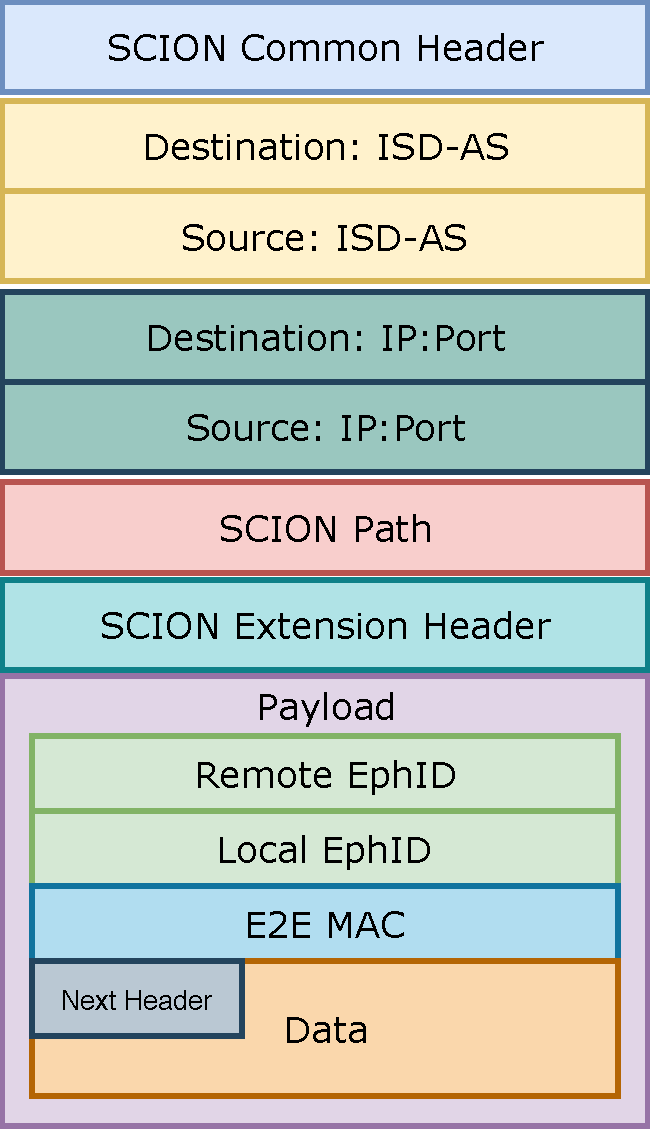
\includegraphics[scale=0.6]{Figures/apna_inside_scion.pdf}}
\decoRule
\caption[APNA packet structure inside SCION]{APNA Packet inside SCION Payload}
\label{fig:apna_scion_pkt}
\end{figure}

Figure \ref{fig:apna_scion_pkt} represents a modified SCION packet encapsulating APNA packet inside it as a payload. IP addresses shown in the above packet are filled with random address while constructing the packet.

\subsection{SNET}
Since we no longer wants to use IP address for our communication the main networking library needs to be modified to accommodate that request. In order to accomplish this \texttt{snet.ListenSCION()} and \texttt{snet.DialSCION()} needs a accept a new network string parameter "\texttt{apna}". Before this it only supported "\texttt{udp4}". Accordingly the \texttt{read} and \texttt{write} methods provided by interface \texttt{snet.Conn} also needs to be modified as they deal with creating and parsing the SCION packet. Currently IP address for source and destination are set to actual ones corresponding to the host. But since we want to hide those IP addresses we can redact it with some random address as its not needed for intra-domain forwarding. For inter-domain forwarding last hop border router fills in with the correct IP address.

\subsubsection{APNA Session Management}
APNA session consists of following components:
\begin{itemize}
    \item \texttt{SessionPrivateKey}:  This private key corresponds two second EphID which contributes to the SessionSecret.
    \item \texttt{SessionSharedSecret}: This shared secret key derived from the pair of second EphID public/private key pairs.
    \item \texttt{PreSessionSharedSecret}: This shared secret key derived from the pair of first EphID public/private key pairs.
    \item \texttt{LocalEphID}: is the host's session EphID
    \item \texttt{RemoteEphID}: is the session EphID of the remote host.
\end{itemize}

\subsubsection{APNA Key Exchange inside SNET}
Since the underlying network is still UDP based, so SNET needs to implement the handshake on top this UDP based overlay network. The goal of this handshake is to initialize the aforementioned session structure. In the first part of the handshake \texttt{PreSessionSharedSecret} and  \texttt{SessionPrivateKey} gets populated and in the second part of the handshake rest of the parameters gets initialized.

\section{Data Communication} \label{overlay:comm}
In order to communicate on the network, a host needs to initialize the networking context with snet and register its IP address with dispatcher. Once a host is successfully registered with dispatcher it can contact the APNA Management Service to issue an Session EphID to the host. Then the host will contact the DNS service to obtain the EphID of the server that it wants to talk to. After that host could initialize the APNA handshake by creating the first APNA packet. When the SCION packet is constructed L4 src and dst address are filled with random bytes and in the payload you can find the APNA packet. When the border router at the src AS gets that packet. It performs some local processing to convert payload back to APNA Packet and perform MAC verification before forwarding it to the neighbouring BR mentioned in path information.

\subsection{Data Forwarding}
A border router in the source AS ensures that only packets from authenticated hosts and authorized EphIDs leave the AS; and a border router in the destination AS forwards the packets to correct dispatcher based on the destination EphID. Transit ASes do not perform additional operations and simply forward the packets to the next AS mentioned in the SCION header path information. In order to achieve high performance data forwarding, only symmetric cryptographic operations are used.

Communication end-points are specified as ISD-AS:EphID tuples. For inter-domain forwarding, border routers use only ISD-AS to forward packets. Specifically, for external packets entering the AS, a border router checks whether the packet has arrived at the destination AS (Figure \ref{fig:overlay_dst}). If not, the packet is forwarded to the next AS mentioned in the Path Information in the SCION packet (Line 9). At the destination AS, the border router performs the following conditions: 1) the destination EphID ($EphID_{d}$) is valid, i.e., has not expired (Line 4).

If all the conditions are satisfied, then the border router tries to resolve IP address from $HID_{d}$ with the help of APNA Management Service. First border check its own cache of IP address from HID, if the HID is not present in its cache it would sent a host resolution query to the APNA management service. If the APNA Management Service replies with $ErrHostNotPresent$ it drops the packet and abort. If it replies with $ErrorOK$, then border router forwards the packet to the dispatcher by setting the destination IP address with the reply sent from Management Service. Then the dispatcher forwards the packet according to the host mapping it has depending upon the host which registered with it in the first step.

For outgoing packets, a border router forwards the packet to a neighboring AS only if all the following conditions are satisfied: 1) the source EphID ($EphID_{s}$) is valid i.e., has not expired (Line 3 in the \ref{fig:overlay_src}) 2) the MAC in the packet is correct (Line 6).

To verify the MAC in the packet, a border router retrieves the shared key ($k_{HA}$) between the source host and the AS by searching the host information database ($host\_info$). Entries in this database are populated with the help of APNA Management Service using its Key Management Service (\ref{sec:kms})

\begin{figure}[th!!]
\centering
\hspace*{2cm}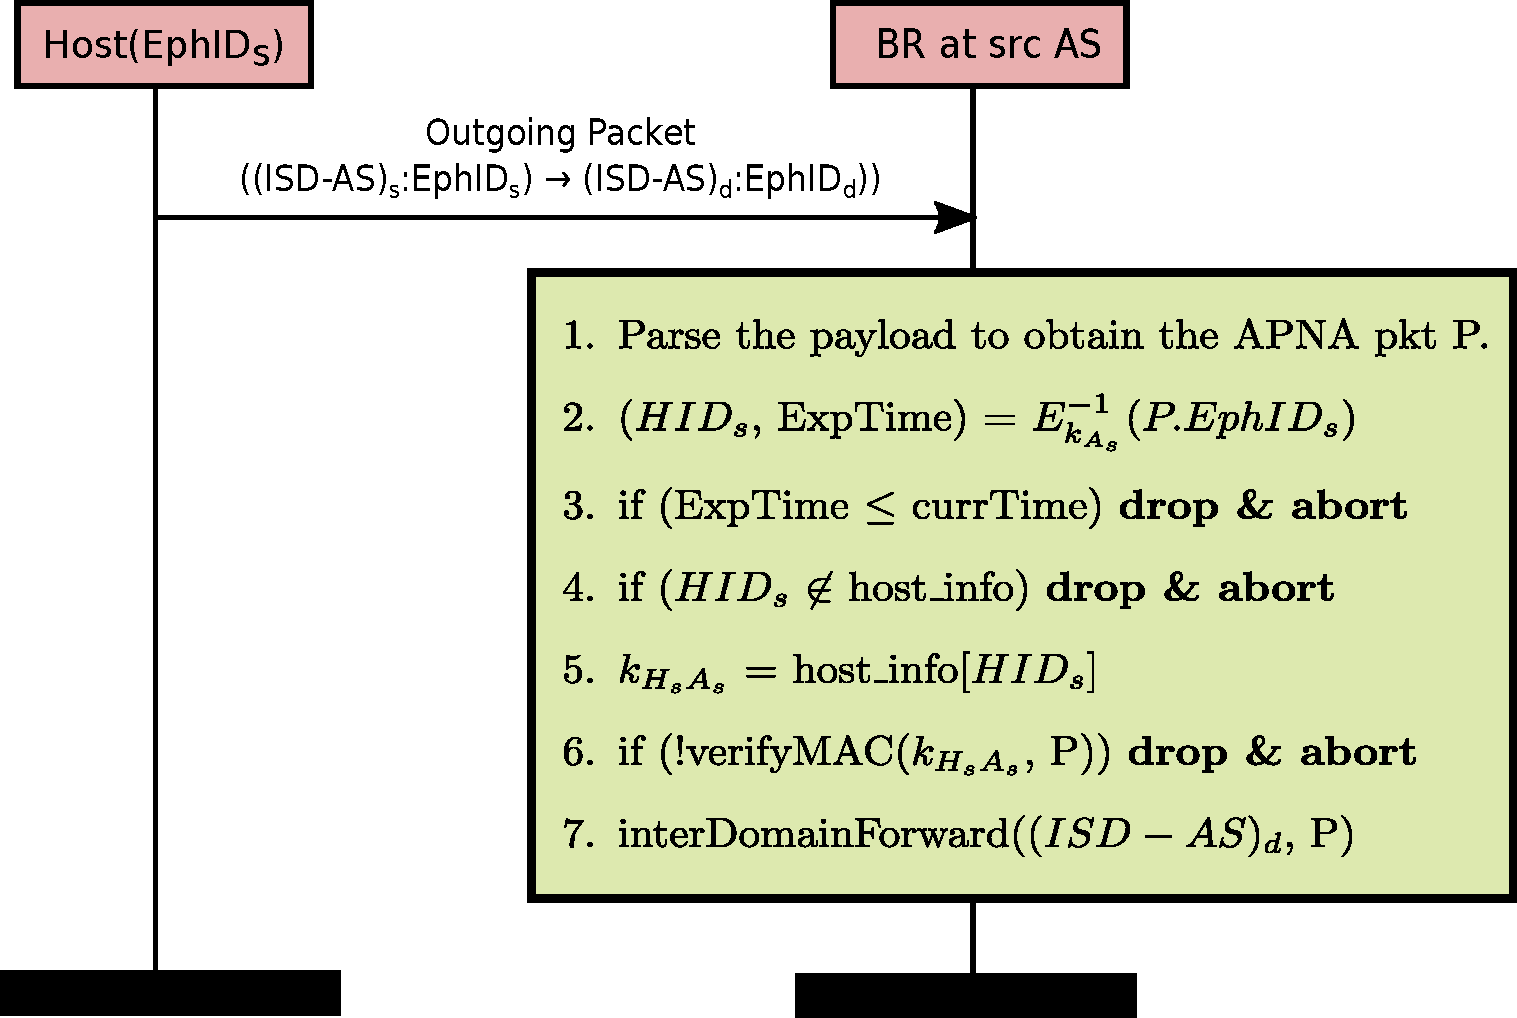
\includegraphics[scale=0.5]{Figures/overlay_src.pdf}
\decoRule
\caption[Apna Overlay Outgoing Packet]{Outgoing Packet}
\label{fig:overlay_src}
\end{figure}

\begin{figure}[th!!]
\centering
\hspace*{2cm}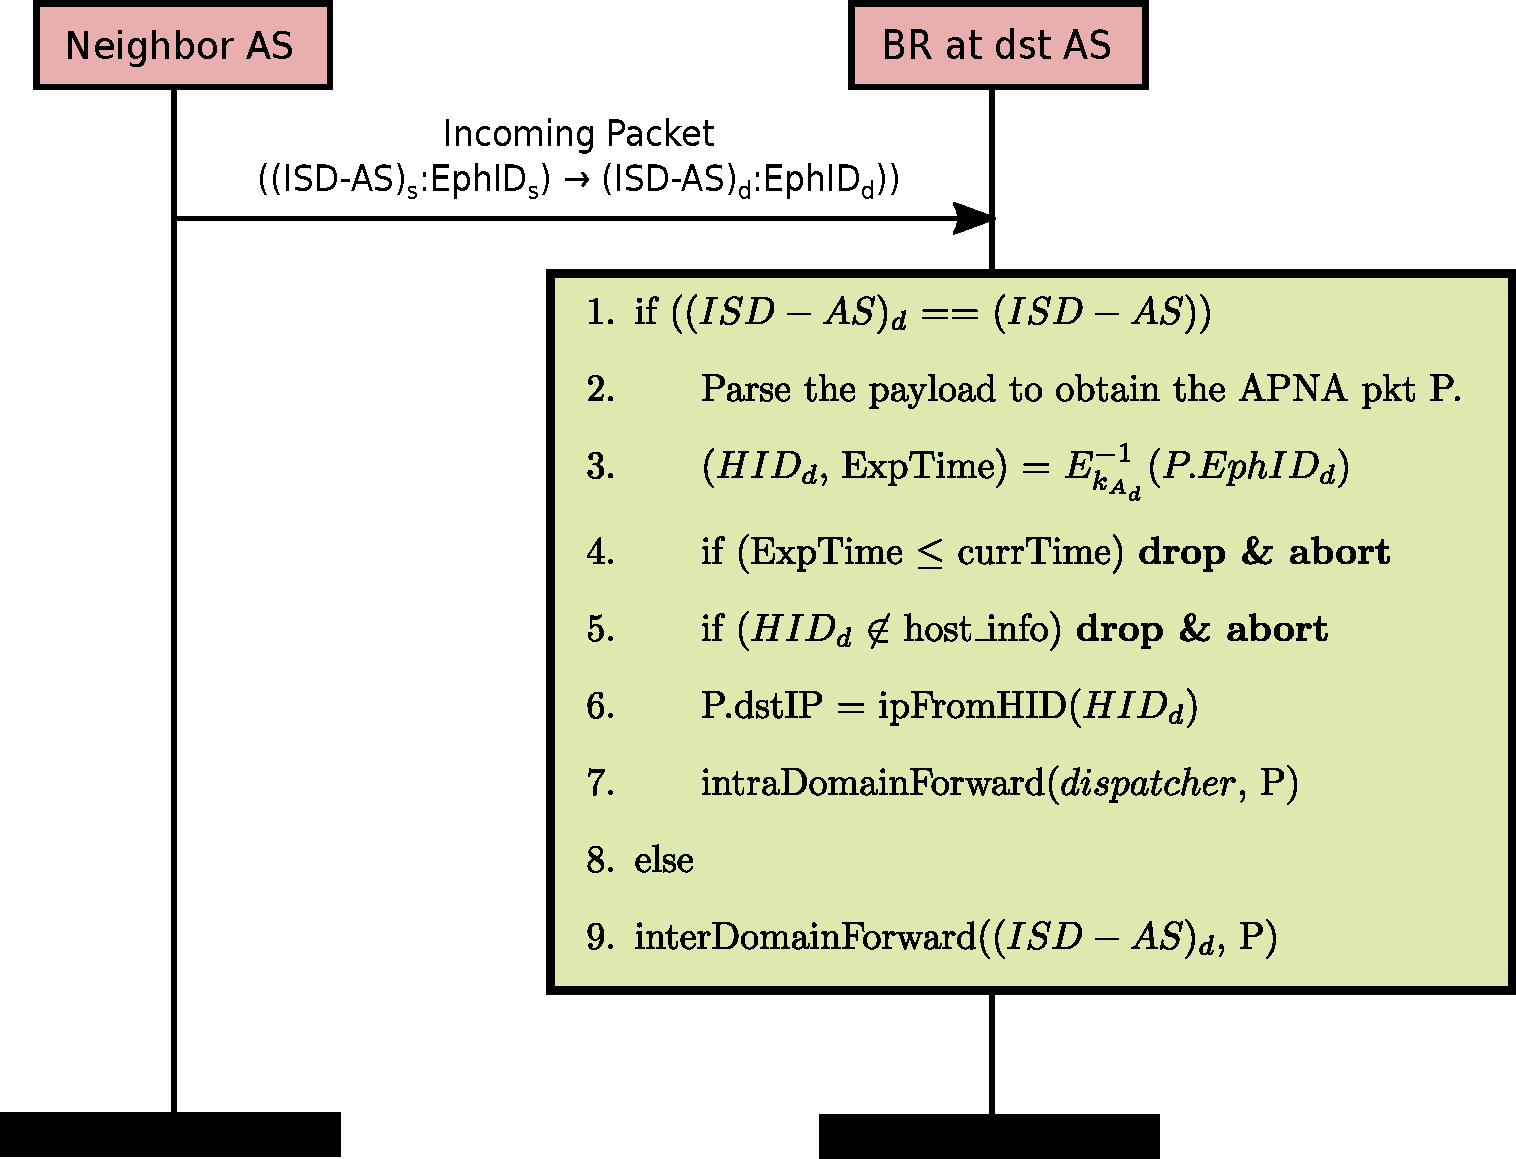
\includegraphics[scale=0.5]{Figures/overlay_dst.pdf}
\decoRule
\caption[Apna Overlay Incoming Packet]{Incoming Packet}
\label{fig:overlay_dst}
\end{figure}

\section{Drawbacks} \label{overlay:drawback}
